\documentclass[12]{article}
\usepackage{listings}
\usepackage{color}
\usepackage{tikz}
\usepackage{amsmath, amsthm, amssymb}
\usetikzlibrary{positioning,shapes,shadows,arrows}

\usepackage{hyperref}
\hypersetup{
  colorlinks=true,
  linkcolor=blue,
  filecolor=magenta,      
  urlcolor=cyan,
}


\title{Neurotic basketball player}
\author{Brett Jackson}

\begin{document}
\maketitle
\section{Introduction}
This is an example problem from FiveThirtyEight's ``The Riddler'' column.
The original problem can be found \href{http://fivethirtyeight.com/features/will-the-neurotic-basketball-player-make-his-next-free-throw/}{here}

\section{Problem statement}
A basketball player is practicing free throws, and makes one of his first two.
The coach has to leave the gym to take a phone call, but knows the player
is somewhat neurotic, and the probability he will make the next shot is equal
to the fraction of shots he has made previously in this session.
When the coach comes back, he sees the player make his 99th shot.
What is the probability the player will make the 100th shot as well.

\section{Solution}
Given the player's expected behavior, we know the probability he will make the
100th shot is equal to
\begin{equation}
  P(\text{make 100}) = \frac{H(99)}{99},
\end{equation}
Where $H(N)$ is equal to the number of shot the player has made in the first $N$
attempts.
Furthermore, we know the player makes the 99th shot, so this becomes
\begin{equation}
  P(\text{make 100}) = \frac{H(98)+1}{99}.
\end{equation}
Ultimately, we can find the probability for $H(98)=i$, and take a weighted sum
to determine the probability the player will make the 100th shot.
\begin{equation}
  P(\text{make 100}) =
  \sum_{i=1}^{97}P\left(H\left(98\right)=i\right)\frac{i+1}{99}.
\end{equation}

If we had no information about the 99th shot, we could simply say
$P\left(H\left(98\right)=i\right)=0.5$, but we can do better than that.
For this problem, it is useful to use Bayesian statistics.
\begin{equation}
  P(H(98)=i | \text{made 99}) =
  \frac{P(\text{made 99} | H(98)=i) P(H(98)=i)}{P(\text{made 99})}.
\end{equation}
Looking at each of these terms, we can quickly say
\begin{equation}
  P(\text{made 99}) = \frac{1}{2}.
\end{equation}
We can also note that for shots $N$, where $N \geq 3$, any number of made shots
is equally likely.
Thus,
\begin{equation}
  P(H(N)=i) = \frac{1}{N-1}.
\end{equation}
So, we can say
\begin{equation}
  P(H(98)=i) = \frac{1}{97},
\end{equation}
for all values of $i$ in the range $[1,97]$.

Finally, to tackle the last piece $P(\text{made 99} | H(98)=i) P(H(98)=i)$.
Since the number of made shots in the first 98 is given, this is equal to
\begin{equation}
  P(\text{made 99} | H(98)=i) = \frac{i}{98}.
\end{equation}

Putting this all together, we get
\begin{eqnarray}
  P(\text{make 100})
  & = &
  \sum_{i=1}^{97}\frac{i}{98} \cdot \frac{1}{97} \cdot 2 \cdot \frac{i+1}{99} \\
  & = &
  \frac{2}{99\cdot98\cdot97} \sum_{i=1}^{97}i(i+1) \\
  & = &
  \frac{2}{99\cdot98\cdot97}\left(\sum_{i=1}^{97}i^2 + \sum_{i=1}^{97}i \right).
\end{eqnarray}

These are two known sums, namely
\begin{eqnarray}
  \sum_{i=1}^{N} i & = & \frac{N(N+1)}{2} \\
  \sum_{i=1}^{N} i^2 & = & \frac{N(N+1)(2N+1)}{6}.
\end{eqnarray}

Plugging these identities into the equation, we get
\begin{eqnarray}
  P(\text{make 100})
  & = &
  \frac{2}{99\cdot98\cdot97}
  \left(\frac{97\cdot98}{2} + \frac{98\cdot97\cdot195}{6} \right) \\
  & = &
  \frac{2}{99\cdot98\cdot97} \frac{97\cdot98}{6} \left(3 + 195\right) \\
  & = &
  \frac{2}{99\cdot98\cdot97} \frac{97\cdot98\cdot198}{6} \\
  & = &
  \frac{2}{3}.
\end{eqnarray}

The probability the player makes the 100th shot is $\frac{2}{3}$

\begin{figure}
\begin{center}
  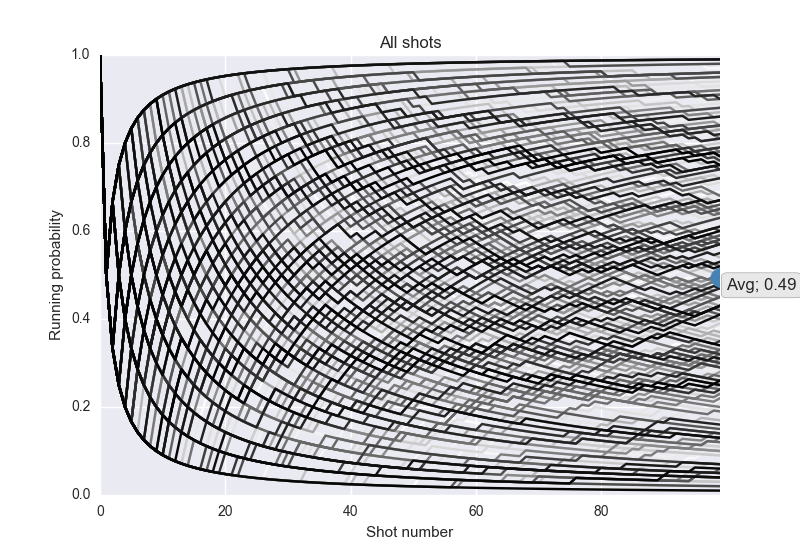
\includegraphics[width=0.9\textwidth]{figs/all_shots.png}
\end{center}
\caption{Running probability for the player to make each shot}
\label{fig:}
\end{figure}

\begin{figure}
\begin{center}
  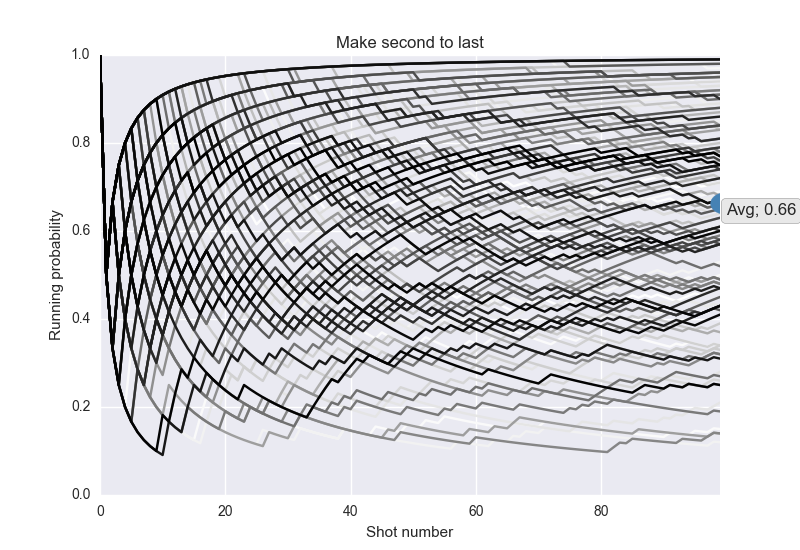
\includegraphics[width=0.9\textwidth]{figs/make_99.png}
\end{center}
\caption{Running probability for the player to make each shot. This plot
         includes only simulations where the player makes the 99th shot.}
\label{fig:}
\end{figure}

\begin{figure}
\begin{center}
  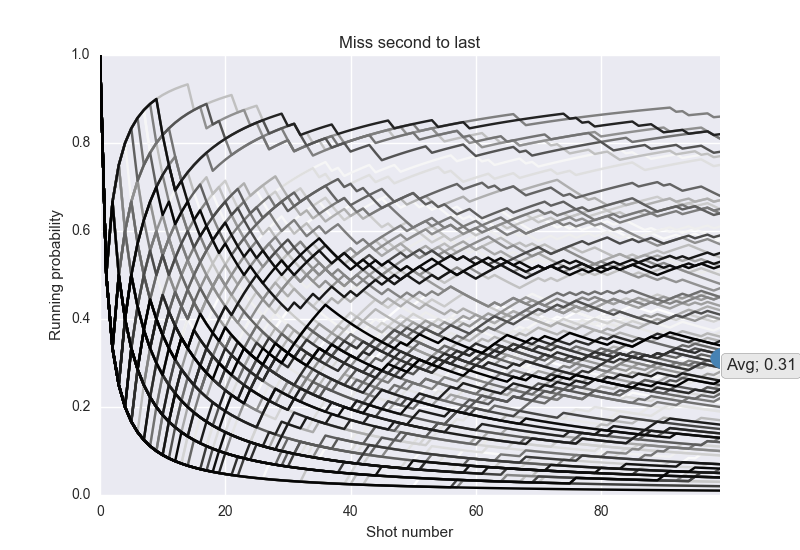
\includegraphics[width=0.9\textwidth]{figs/miss_99.png}
\end{center}
\caption{Running probability for the player to make each shot. This plot
         includes only simulations where the player misses the 99th shot.}
\label{fig:}
\end{figure}


\end{document}
